\def\baselinestretch{1}
\chapter{RESULTS} \label{chap:results}
    \minitoc
    \begin{center}
    	\emph{Abstract of chapter \ref{chap:results}}
    \end{center}
    
    \section{Source list}
    	The list of sources which were studied are listed in table \ref{tab:source-list} below.
    	
    	\renewcommand{\arraystretch}{1.5}
    	\begin{table}[!htb]
    		\centering
    		\caption{List of sources in dataset}
    		\label{tab:source-list}
			\begin{tabular}{cccccc}
			\hline
			\textbf{S. No.} & \textbf{Source} & \textbf{Type} & \textbf{Galaxy} & \textbf{\begin{tabular}[c]{@{}c@{}}R. A.\\ (degrees)\end{tabular}} & \textbf{\begin{tabular}[c]{@{}c@{}}Dec.\\ (degrees)\end{tabular}} \\ \hline
			{1} & {CAL 83} & {} & {} & {85.89233} & {-68.37283} \\
			{2} & {RS Oph} & {} & {} & {267.55483} & {-6.70791} \\
			{3} & {RX J0019.8+2156} & {} & {} & {4.95802} & {21.94783} \\
			{4} & {RX J0527.8-6954} & {} & {} & {81.95345} & {-69.90247} \\
			{5} & {RX J0925.7-4758} & {} & {} & {141.44167} & {-47.97148} \\
			{6} & {V3890 Sgr} & {} & {} & {277.68037} & {-24.01915} \\ \hline
			\end{tabular}
		\end{table}
		\renewcommand{\arraystretch}{2.2}
		
		\subsection{Count rates}		
			The count rates of the sources as observed by the respective observatories in table *** over the respective energy ranges are presented in the sub-figures in \ref{result:count-rate}.
			\begin{figure}[h!]
				\centering
				\caption{Count rates of individual sources in dataset}
				\label{result:count-rate}
				\subfloat[CAL 83 \label{count-rate:cal83}]{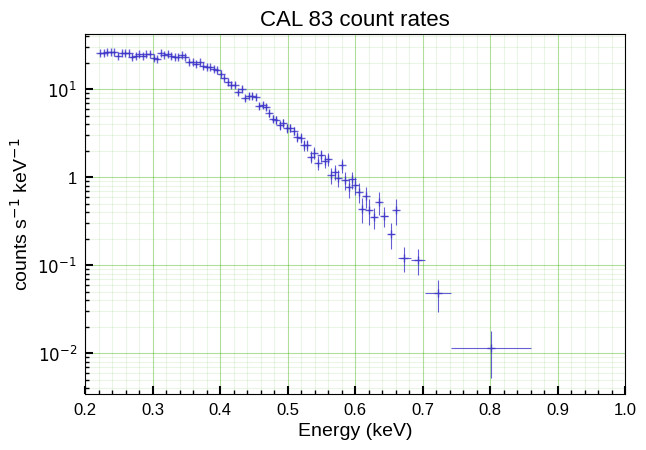
\includegraphics[width=0.45\textwidth]{counts/cal-83-pn_counts}} %\hfill
				\subfloat[RS Oph \label{count-rate:rsoph}]{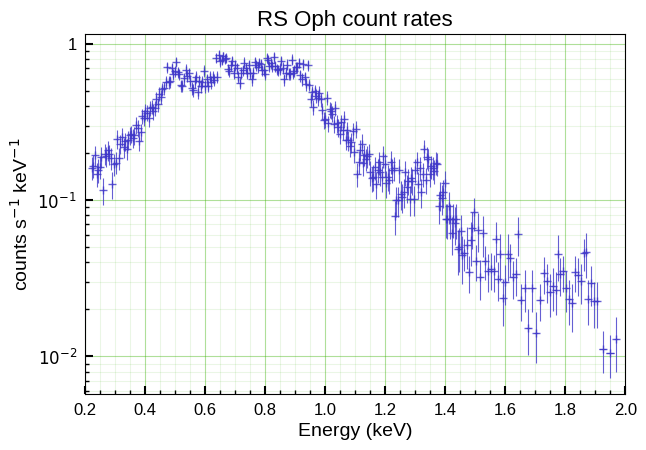
\includegraphics[width=0.45\textwidth]{counts/rs-oph-pn_counts}} %\hfill
				
				\subfloat[RX J0019.8+2156 \label{count-rate:rxj0019}]{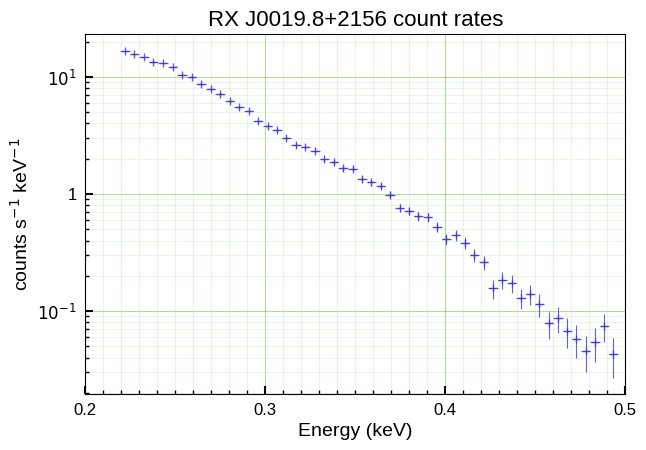
\includegraphics[width=0.45\textwidth]{counts/rx-j0019d8p2156-pn_counts}} %\hfill
				\subfloat[RX J0527.8-6954 \label{count-rate:rxj0527}]{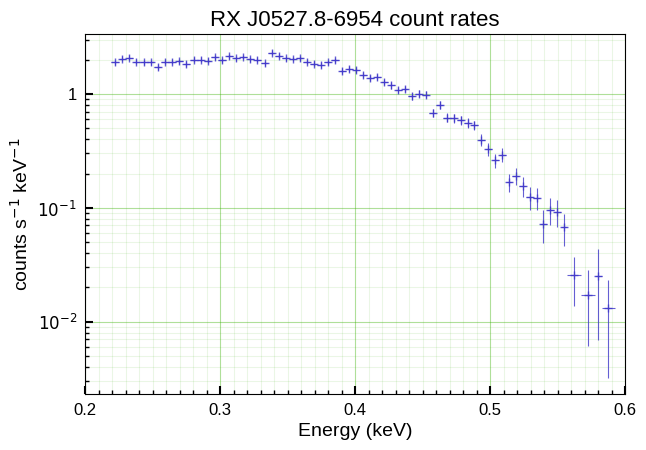
\includegraphics[width=0.45\textwidth]{counts/rx-j0527d8-6954-pn_counts}} %\hfill
				
				\subfloat[RX J0925.7-4758 \label{count-rate:mrvel}]{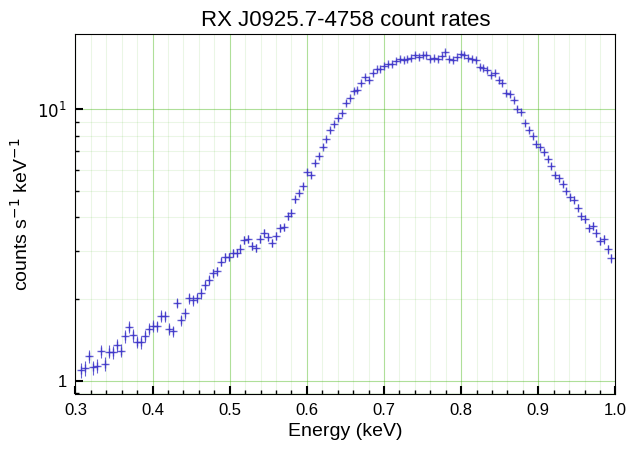
\includegraphics[width=0.45\textwidth]{counts/rx-j0925-4758-pn_counts}} %\hfill
				\subfloat[V3890 Sgr \label{count-rate:v3890}]{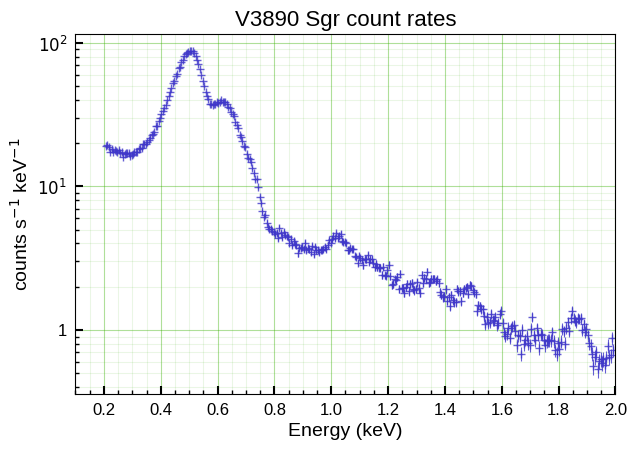
\includegraphics[width=0.45\textwidth]{counts/v3890-sgr-pn_counts}} %\hfill
			\end{figure}
			
			\begin{figure}[h!]
				\centering
				\caption{Count rates of all sources in dataset}
				\label{result:count-rate}
				\subfloat[Count rates of all sources \label{count-rate:cal83}]{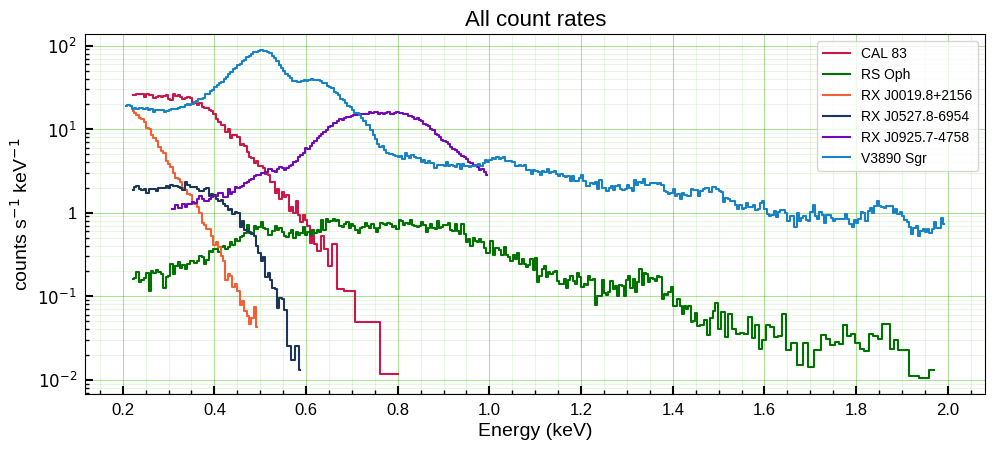
\includegraphics[width=0.8\textwidth]{counts/all_counts}} %\hfill
				
				\subfloat[Normalized count rates of all sources \label{count-rate:rsoph}]{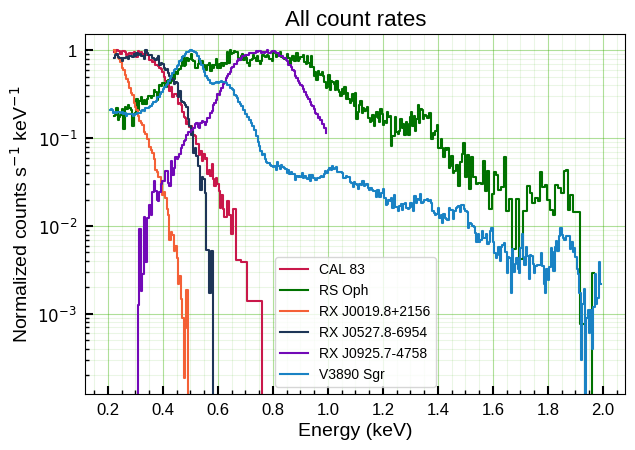
\includegraphics[width=0.8\textwidth]{counts/all_norm-counts}} %\hfill
			\end{figure}
    
%    \section{Spectral Line Identification}
%    
%    \section{XMM-Newton RGS Spectral Fit}
%    The best fit model, i.e. M11, contains two different additive components that simulate optically thin plasma. One of them, i.e. \texttt{apec} uses line lists from the AtomDB database, while the other, i.e. \texttt{mekal} which is based on calculations by Mewe, Kaastra and Liedahl \cite{meka,liedahl}. The latter could indicate the presence of a hot corona. The presence of the \texttt{rauch} model component in the best fit model suggests a substantial contribution due to an NLTE stellar atmosphere. The model also consists of the \texttt{swind1} component, which simulates the presence of a stellar wind component along the line-of-sight. The presence of all the above model components vindicates our hypothesis of the inclusion of non-steady states, NLTE and stellar winds in the radiative processes in X-ray binary systems such as those of RX J0925.7-4758.
%    
%    \section{P Cygni Profiling}